\section*{Question 4}
\begin{figure}[h]
    \centering
    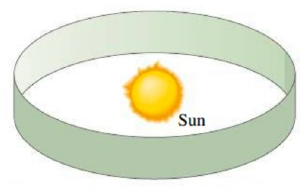
\includegraphics[scale=0.6]{figures/q4.PNG}
\end{figure}
\noindent
A science-fiction story describes an artificial ``planet'' in the form of a band completely encircling a sun, as in the figure. The inhabitants live on the interior surface (where it is always noon). Imagine that this sun is exactly like our own, that the distance to the band is the same as the Earth-Sun distance and that the ring rotates sufficiently quickly to produce an apparent gravity of $g$, as on Earth. What will be the period of revolution, i.e., this planet's year, in terms of the following quantities? 

\begin{itemize}
    \item $g$: Gravitational acceleration on the Earth
    \item $r$: Distance from the sun to the ring-planet
    \item $M$: Mass of the sun
    \item $G$: Universal gravitational constant
    \item Gravitational force between masses $M$ and $m$ : $F=G\frac{Mm}{r^2}$
\end{itemize}

\section*{Solution:}